\documentclass{beamer}
\usetheme{Boadilla}
\usecolortheme{dove}
\usepackage{graphicx}
\usepackage{hyperref}
\usepackage{booktabs}
\usepackage{textcomp}
\usepackage{gensymb}
\usepackage{amsmath} 
\usepackage{microtype}
\usepackage{float}
\graphicspath{{../figures/}}

\title{
  Studying the Effect of Natural Disasters on Economic Activity:\\
  \large{A first Approach using Night-Time Luminosity Data}
}
\author{Cameron, M. \and Rosales, V. \and Westermann, J.P.}

\date{July 30, 2017}

\begin{document}

\begin{frame}
  \maketitle
\end{frame}

\begin{section}{Data}
  \begin{frame}
    \begin{figure}
      \centering
      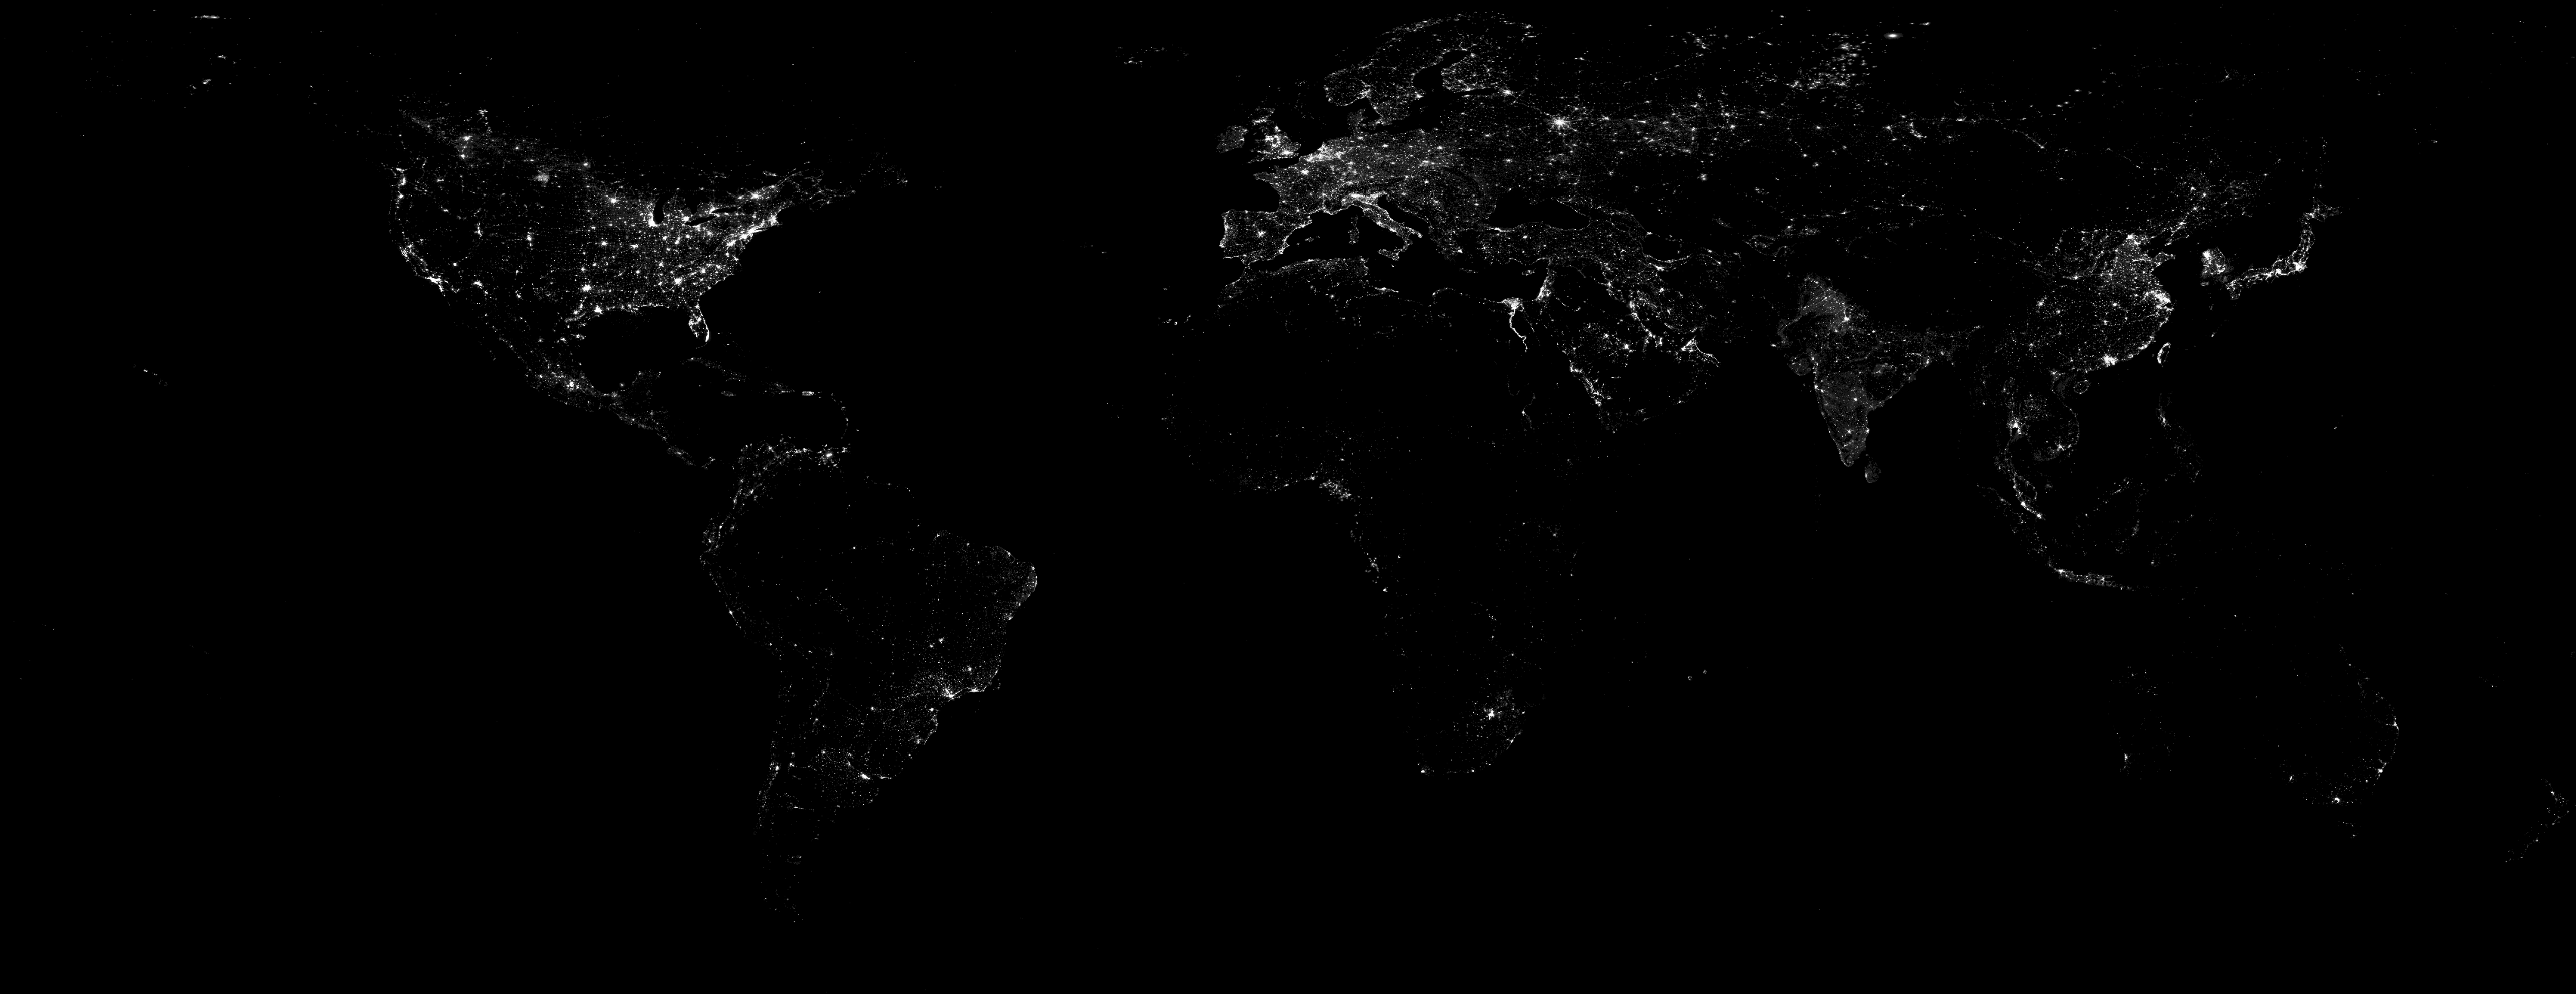
\includegraphics[width=1\linewidth]{lum_2013}\label{lum_2013}
    \end{figure}			
  \end{frame}
\end{section}

\begin{section}{Case Studies}
  \begin{frame}
    \begin{figure}
      \centering
      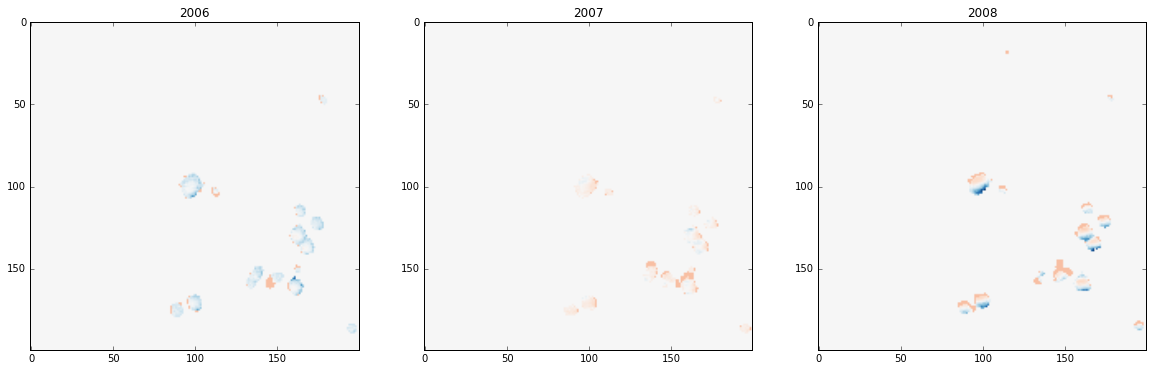
\includegraphics[width=.7\linewidth]{tocopilla_series}\label{fig:tocopilla_series}
      \caption{Absolute change in luminosity in Tocopilla}
      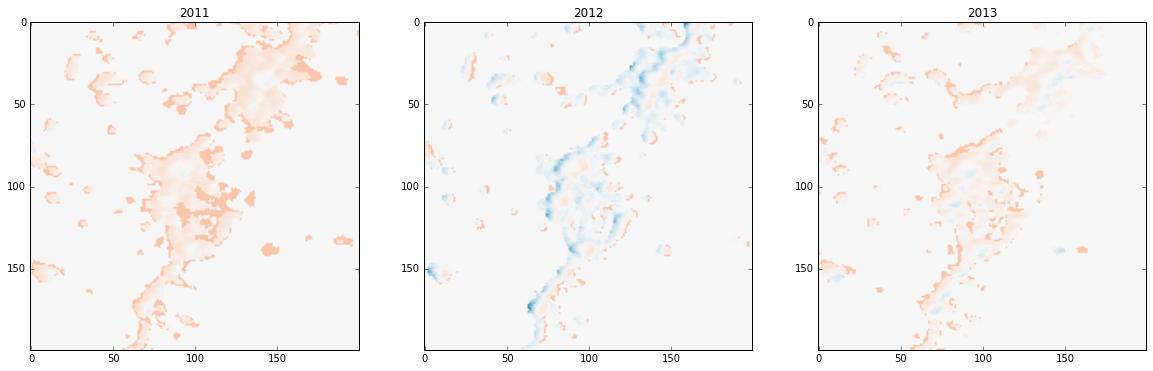
\includegraphics[width=.7\linewidth]{maule_series}\label{fig:maule_series}
      \caption{Absolute change in luminosity in Maule}
    \end{figure}
  \end{frame}

  \begin{frame}
        \begin{figure}
          \centering
          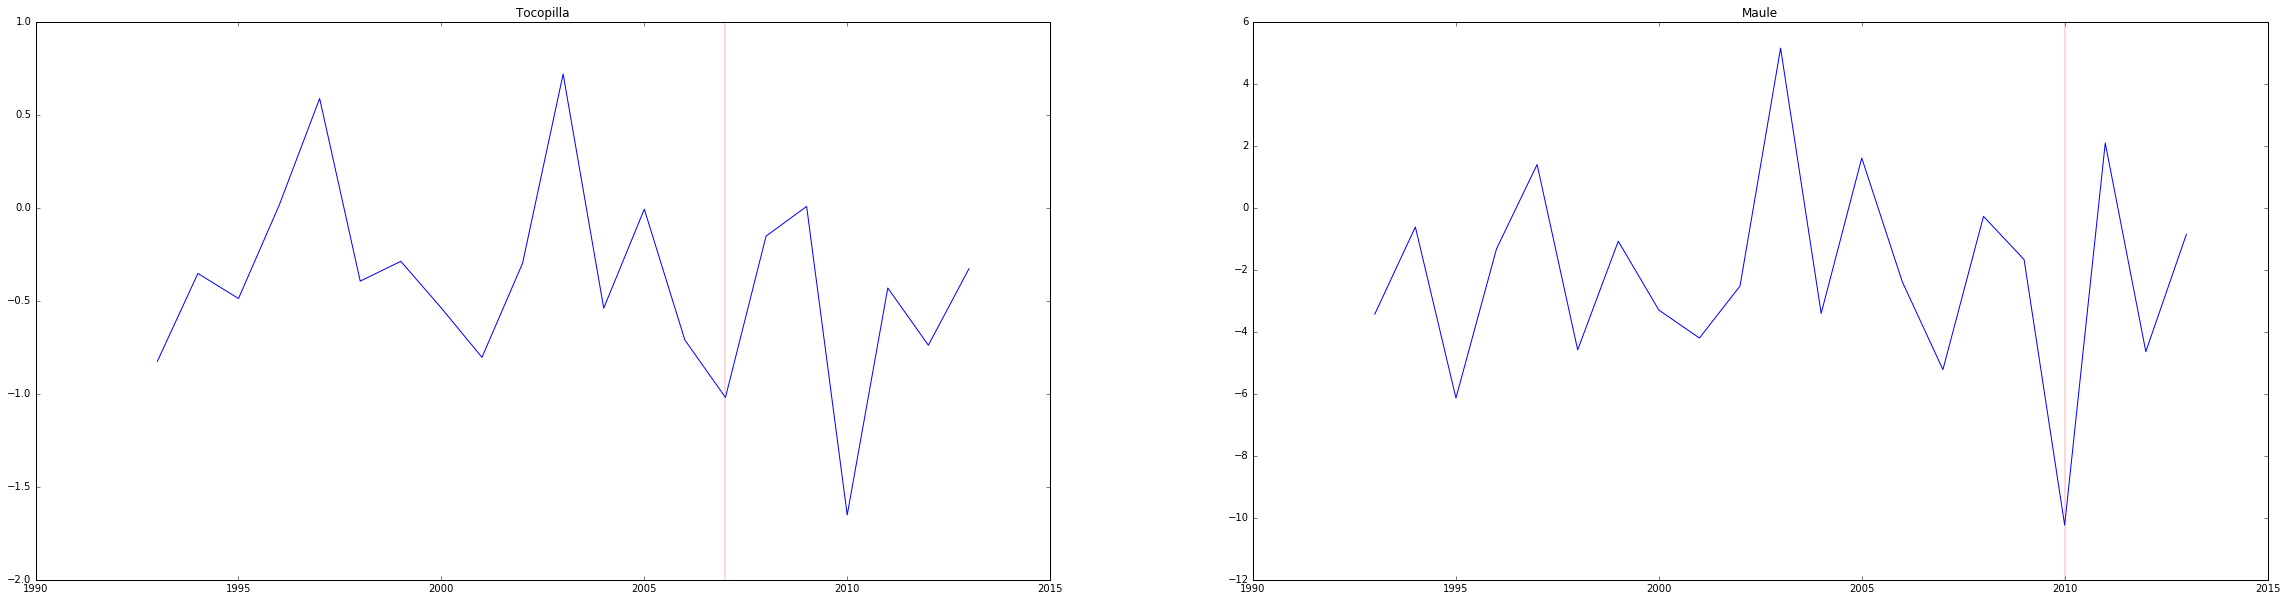
\includegraphics[width=1\linewidth]{maule_tocopilla}\label{fig:maule_tocopilla}
          \caption{Tocopilla and Maule Luminosity Sum Time Series}
        \end{figure}
  \end{frame}

  \begin{frame}
        \begin{figure}
          \centering
          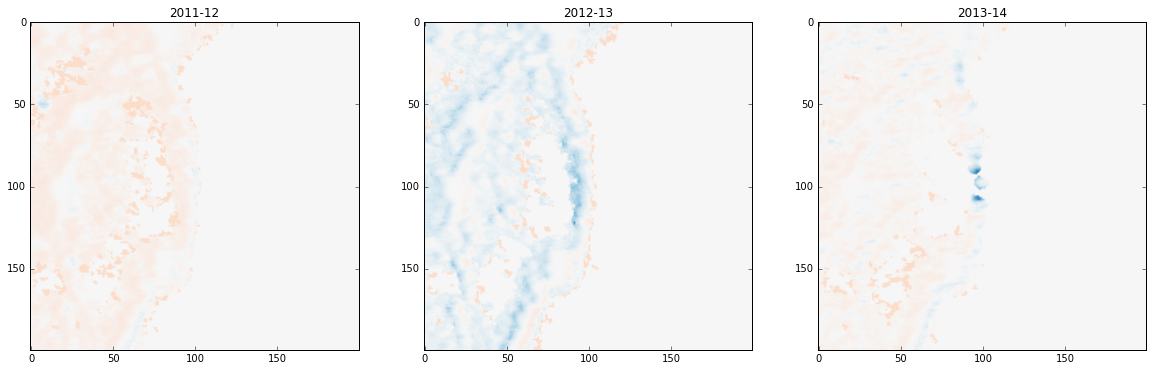
\includegraphics[width=1\linewidth]{fukushima}\label{fig:fukushima}
          \caption{Fukushima Luminosity Delta around Tsunami Occurance}
        \end{figure}
  \end{frame}
\end{section}

\begin{section}{Modelling}
  \begin{frame}{Modelling Earthquake Impact Linearly Decaying with Distance}{Disco vs. Luminosity}
    \begin{figure}
      \centering
      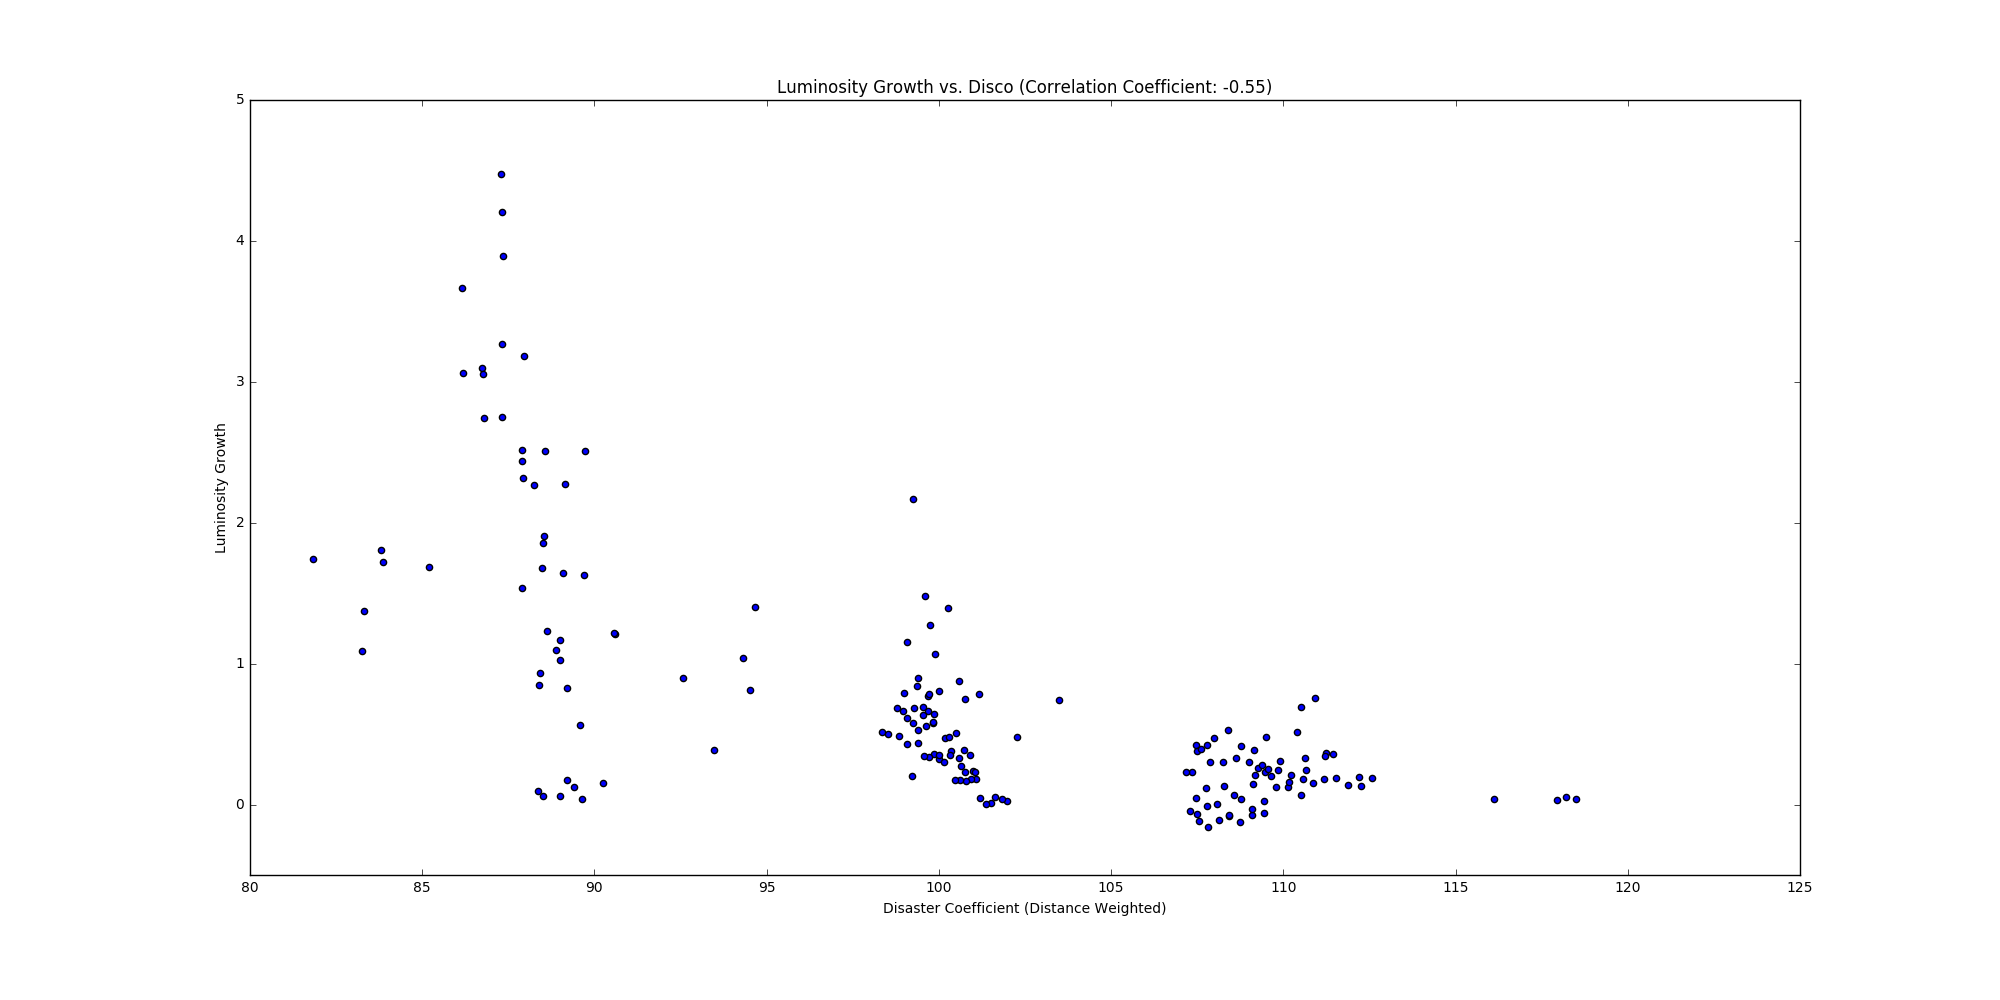
\includegraphics[width=1\linewidth]{linear-lum-vs-disco}\label{fig:linear-model-disco-vs-lum-growth} %TODO: Adjust plot pngs to have sensible size for document
      \caption{Luminosity Growth 1992-2013 plotted against a linearly decaying disaster coefficient for 150x150 image sections.}
    \end{figure}
  \end{frame}

  \begin{frame}{Modelling Earthquake Impact based on Institutional Reports}{Earthquake Lag Coefficients}
    \begin{figure}
      \centering
      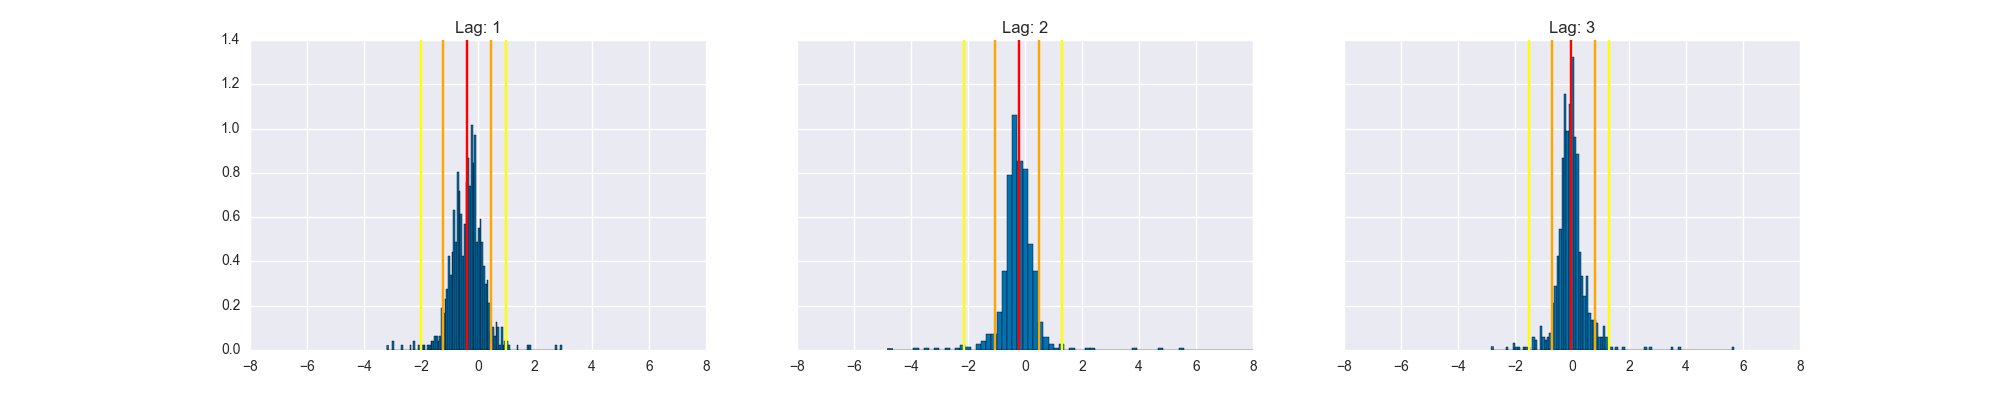
\includegraphics[width=\linewidth]{non_balanced_earthquake_coefficients_distribution}\label{fig:non_balanced_earthquake_coefficients_distribution}
      \caption{Distribution of Lag Coefficients for Earthquakes in Vector Autoregression Models per City with 95th and 99th Percentiles}
    \end{figure}
  \end{frame}

  \begin{frame}{Modelling Earthquake Impact based on Institutional Reports}{Earthquake Lag Coefficients}
    \begin{figure}
      \centering
      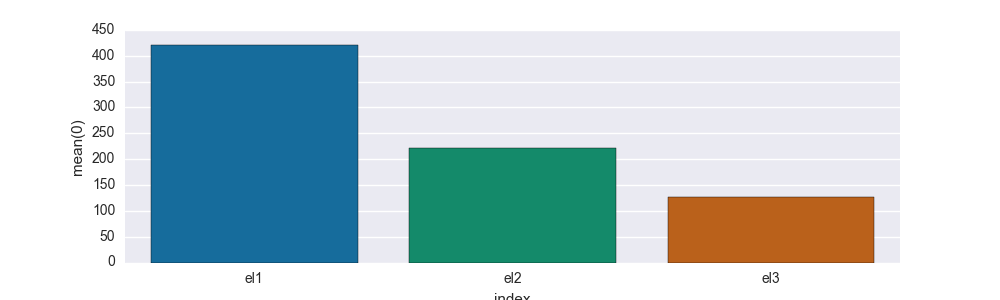
\includegraphics[width=\linewidth]{non_balanced_earthquake_coefficients_winning_lag}\label{fig:non_balanced_earthquake_winning_lag}
      \caption{Count of the most impactful earthquake lag coefficient across all cities}
    \end{figure}
  \end{frame}

  \begin{frame}{Panel Model}{Region Series}
    \begin{figure}
      \centering
      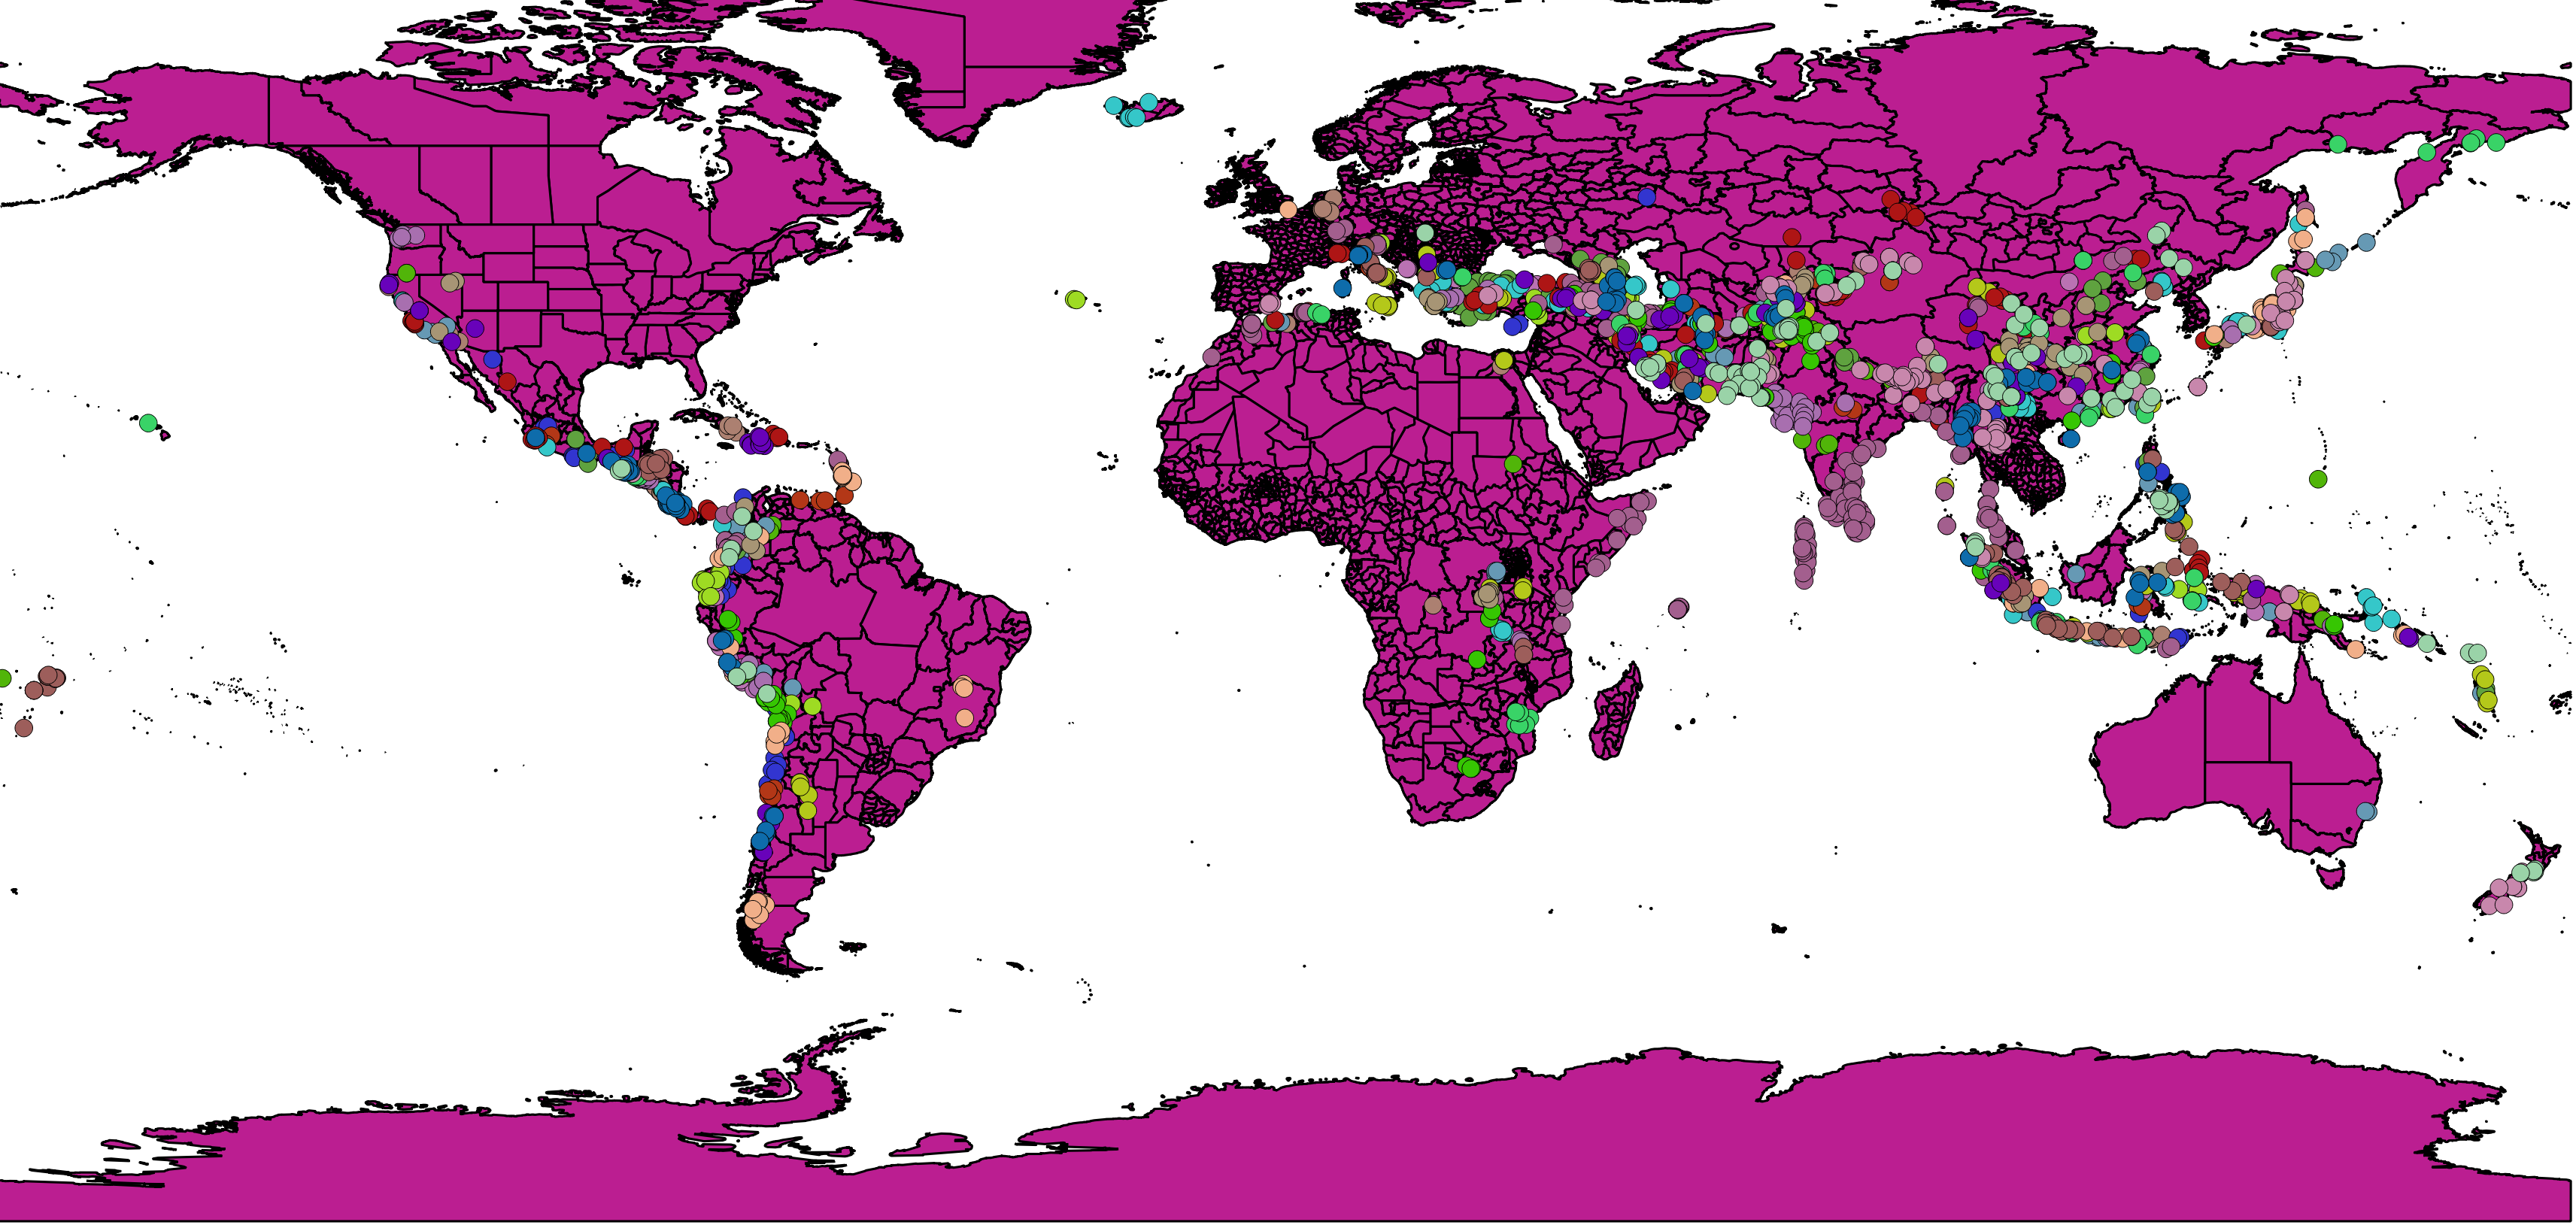
\includegraphics[width=1\linewidth]{world_regions}
      \caption{Administrative regions and earthquakes}\label{eq}
    \end{figure}
  \end{frame}

  \begin{frame}{Panel Model}{Section Series}
    \begin{figure}
      \centering
      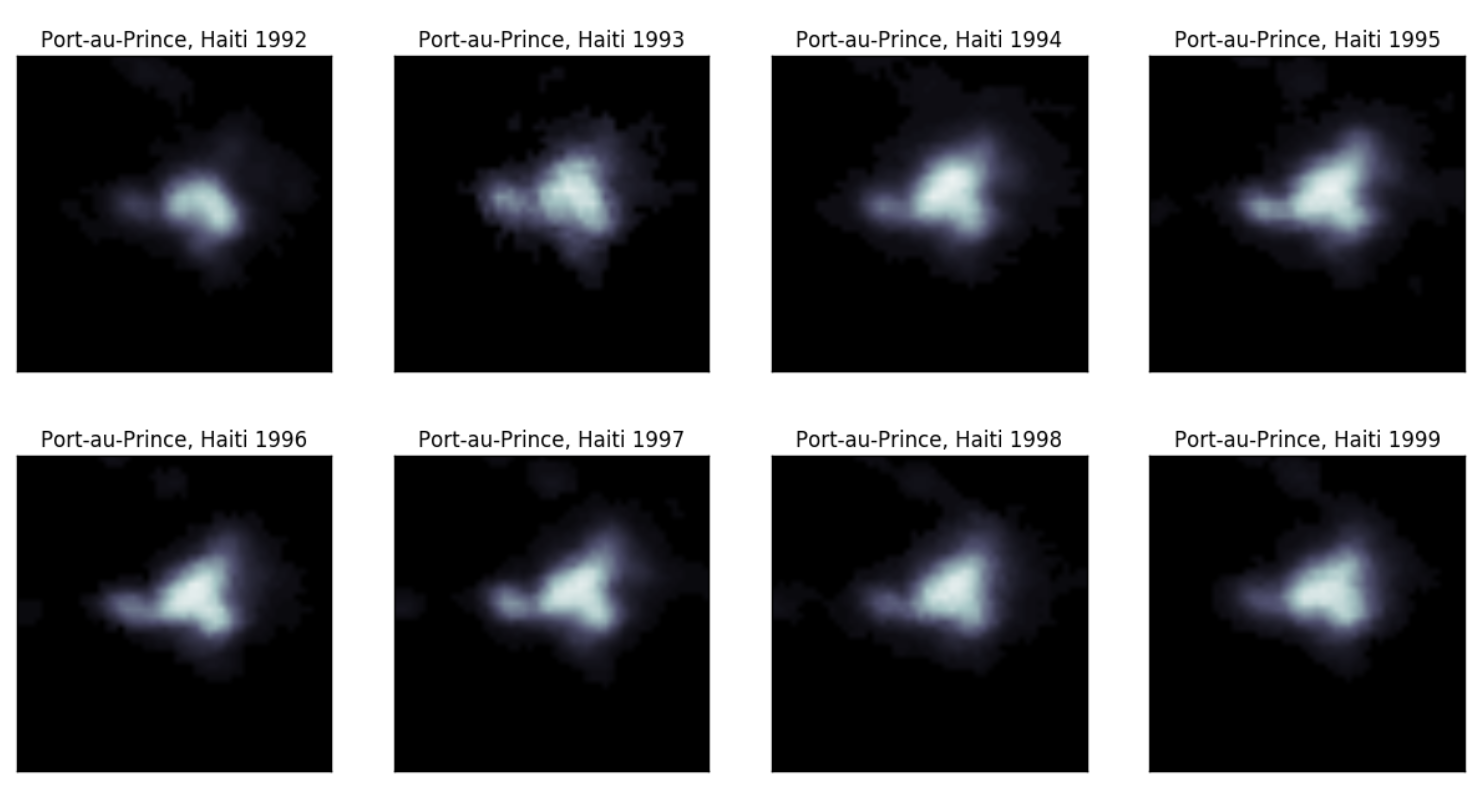
\includegraphics[width=\linewidth]{haiti_luminosity_series_short}\label{fig:haiti_luminosity_series_short}
      \caption{50x50 pixel atellite image cutout of Port-au-Prince, Haiti}
    \end{figure}
  \end{frame}

  \begin{frame}{Dynamic Panel Model with Fixed Effects}{Formula}
    \begin{align*}
      y_{i,t}-y_{i,t-1}=\alpha_i+\beta_t+\gamma(y_{i,t-1}-y_{i,t-2})+\delta EQ_{i,t}+\eta EQ_{i,t-1}+\epsilon_{i,t}
    \end{align*}      
  \end{frame}
\end{section}

\begin{section}{Results}
  \begin{frame}{City-level Dynamic Panel Regression}
    % \begin{table}
    %   \centering
    %   %\begin{tiny}
    %   \def\sym#1{\ifmmode^{#1}\else\(^{#1}\)\fi}
    %   \caption{Regression using cities data, separated by geographic regions(all the events)\label{tab3}}
    %   \resizebox{\textwidth}{!}{
    %     \begin{tabular}{l*{8}{c}}
    %       \hline\hline
    %       &\multicolumn{1}{c}{World}&\multicolumn{1}{c}{E. Asia \&}&\multicolumn{1}{c}{Europe \&}&\multicolumn{1}{c}{LA \&}&\multicolumn{1}{c}{ME \& N}&\multicolumn{1}{c}{North}&\multicolumn{1}{c}{South}&\multicolumn{1}{c}{Sub-Saharan}\\
    %       &\multicolumn{1}{c}{}&\multicolumn{1}{c}{Pacific}&\multicolumn{1}{c}{C. Asia}&\multicolumn{1}{c}{Caribbean}&\multicolumn{1}{c}{Africa}&\multicolumn{1}{c}{America}&\multicolumn{1}{c}{Asia}&\multicolumn{1}{c}{Africa}\\
    %       \hline
    %       lum\_gr\_1            &      -0.400\sym{**}&      -0.427\sym{**}&      -0.410\sym{**}&      -0.387\sym{**}&      -0.271\sym{**}&      -0.445\sym{**}&      -0.317\sym{**}&      -0.359\sym{**}\\
    %                             &   (-415.58)        &   (-160.80)        &   (-290.78)        &   (-162.52)        &    (-23.47)        &   (-138.06)        &    (-88.81)        &    (-66.85)        \\
    %       [1em]
    %       eq    &    -0.00772        &      0.0135        &     -0.0285        &     -0.0313\sym{**}&      0.0114        &      0.0103        &      0.0217        &     -0.0492        \\
    %             &     (-0.86)        &      (0.50)        &     (-1.37)        &     (-2.51)        &      (0.12)        &      (0.25)        &      (0.85)        &     (-0.42)        \\
    %       [1em]
    %       eq\_1  &    -0.00386        &     0.00274        &    -0.00375        &    -0.00698        &     -0.0213        &      0.0370        &     -0.0107        &      -0.136        \\
    %              &     (-0.43)        &      (0.10)        &     (-0.18)        &     (-0.56)        &     (-0.22)        &      (0.96)        &     (-0.40)        &     (-1.16)        \\
    %       \hline
    %       Observations        &      798844        &      104184        &      373310        &      116333        &        6977        &       71460        &       64807        &       26164        \\
    %       \hline\hline
    %       \multicolumn{9}{l}{\footnotesize \textit{t} statistics in parentheses}\\
    %       \multicolumn{9}{l}{\footnotesize \sym{*} \(p<0.10\), \sym{**} \(p<0.05\)}\\
    %   \end{tabular}}
    %   %\end{tiny}
    % \end{table}
  \end{frame}
\end{section}


\begin{section}{Appendix}
  % \begin{frame}{Region-level Data}
  %   \begin{table}\centering
  %     %\begin{tiny}
  %     \def\sym#1{\ifmmode^{#1}\else\(^{#1}\)\fi}
  %     \caption{Regression using regional data, separated by geographic regions (all the earthquakes)\label{tab1}}
  %     \resizebox{\textwidth}{!}{
  %       \begin{tabular}{l*{8}{c}}
  %         \hline\hline
  %         &\multicolumn{1}{c}{World}&\multicolumn{1}{c}{E. Asia \&}&\multicolumn{1}{c}{Europe \&}&\multicolumn{1}{c}{LA \&}&\multicolumn{1}{c}{ME \& N}&\multicolumn{1}{c}{North}&\multicolumn{1}{c}{South}&\multicolumn{1}{c}{Sub-Saharan}\\
  %         &\multicolumn{1}{c}{}&\multicolumn{1}{c}{Pacific}&\multicolumn{1}{c}{C. Asia}&\multicolumn{1}{c}{Caribbean}&\multicolumn{1}{c}{Africa}&\multicolumn{1}{c}{America}&\multicolumn{1}{c}{Asia}&\multicolumn{1}{c}{Africa}\\
  %         \hline
  %         lum\_gr\_1            &      -0.344\sym{**}&      -0.369\sym{**}&      -0.378\sym{**}&      -0.344\sym{**}&      -0.168\sym{**}&      -0.479\sym{**}&      -0.233\sym{**}&      -0.301\sym{**}\\
  %                               &   (-113.60)        &    (-47.16)        &    (-85.28)        &    (-42.27)        &    (-14.67)        &    (-25.88)        &    (-13.16)        &    (-35.62)        \\
  %         [1em]
  %         eq1                 &     0.00957        &     0.00313        &      0.0249        &    -0.00331        &      0.0107        &     -0.0139        &      0.0400        &      0.0352        \\
  %                             &      (1.15)        &      (0.18)        &      (1.60)        &     (-0.26)        &      (0.94)        &     (-0.22)        &      (1.10)        &      (0.46)        \\
  %         [1em]
  %         eq1\_1               &    0.000435        &     -0.0253        &     0.00323        &    -0.00384        &     0.00661        &     -0.0171        &      0.0694\sym{*} &      0.0677        \\
  %                              &      (0.05)        &     (-1.39)        &      (0.21)        &     (-0.30)        &      (0.57)        &     (-0.28)        &      (1.88)        &      (0.96)        \\
  %         \hline
  %         Obs.        &       86126        &       13337        &       37588        &       11089        &        7481        &        2215        &        2621        &       11795        \\
  %         \hline\hline
  %         \multicolumn{9}{l}{\footnotesize \textit{t} statistics in parentheses}\\
  %         \multicolumn{9}{l}{\footnotesize \sym{*} \(p<0.10\), \sym{**} \(p<0.05\)}\\
  %     \end{tabular}}
  %     %\end{tiny}
  %   \end{table}
  % \end{frame}

  % \begin{frame}{Region-level Data}{Big Earthquakes}
  %   \begin{table}\centering
  %     %\begin{tiny}
  %     \def\sym#1{\ifmmode^{#1}\else\(^{#1}\)\fi}
  %     \caption{Regression using regional data, separated by geographic regions (using only big earthquakes)\label{tab2}}
  %     \resizebox{\textwidth}{!}{
  %       \begin{tabular}{l*{8}{c}}
  %         \hline\hline
  %         &\multicolumn{1}{c}{World}&\multicolumn{1}{c}{E. Asia \&}&\multicolumn{1}{c}{Europe \&}&\multicolumn{1}{c}{LA \&}&\multicolumn{1}{c}{ME \& N}&\multicolumn{1}{c}{North}&\multicolumn{1}{c}{South}&\multicolumn{1}{c}{Sub-Saharan}\\
  %         &\multicolumn{1}{c}{}&\multicolumn{1}{c}{Pacific}&\multicolumn{1}{c}{C. Asia}&\multicolumn{1}{c}{Caribbean}&\multicolumn{1}{c}{Africa}&\multicolumn{1}{c}{America}&\multicolumn{1}{c}{Asia}&\multicolumn{1}{c}{Africa}\\
  %         \hline
  %         lum\_gr\_1            &      -0.344\sym{**}&      -0.369\sym{**}&      -0.378\sym{**}&      -0.344\sym{**}&      -0.168\sym{**}&      -0.479\sym{**}&      -0.232\sym{**}&      -0.301\sym{**}\\
  %                               &   (-113.59)        &    (-47.16)        &    (-85.27)        &    (-42.27)        &    (-14.64)        &    (-25.89)        &    (-13.08)        &    (-35.64)        \\
  %         [1em]
  %         eq2                 &    -0.00363        &     -0.0439        &      0.0190        &     0.00675        &      0.0789\sym{*} &           0        &      0.0471        &      0.0326        \\
  %                             &     (-0.18)        &     (-1.02)        &      (0.41)        &      (0.23)        &      (1.65)        &         (.)        &      (0.65)        &      (0.29)        \\
  %         [1em]
  %         eq2\_1               &     -0.0303        &     -0.0507        &      -0.109\sym{**}&     -0.0250        &     -0.0547        &           0        &     0.00537        &       0.113        \\
  %                              &     (-1.41)        &     (-1.07)        &     (-2.37)        &     (-0.84)        &     (-1.15)        &         (.)        &      (0.07)        &      (1.02)        \\
  %         \hline
  %         Obs.        &       86126        &       13337        &       37588        &       11089        &        7481        &        2215        &        2621        &       11795        \\
  %         \hline\hline
  %         \multicolumn{9}{l}{\footnotesize \textit{t} statistics in parentheses}\\
  %         \multicolumn{9}{l}{\footnotesize \sym{*} \(p<0.10\), \sym{**} \(p<0.05\)}\\
  %     \end{tabular}}
  %     %\end{tiny}
  %   \end{table}
  % \end{frame}

  % \begin{frame}{Region-level Data}{Income Groups}
  %   \begin{table}\centering
  %     \def\sym#1{\ifmmode^{#1}\else\(^{#1}\)\fi}
  %     \caption{Regression using regional data, separated by income groups (all the events)\label{tab4}}
  %     \begin{tabular}{l*{4}{c}}
  %       \hline\hline
  %       &\multicolumn{1}{c}{Low}&\multicolumn{1}{c}{Lower Middle}&\multicolumn{1}{c}{Upper Middle}&\multicolumn{1}{c}{High}\\
  %       &\multicolumn{1}{c}{lum\_gr}&\multicolumn{1}{c}{lum\_gr}&\multicolumn{1}{c}{lum\_gr}&\multicolumn{1}{c}{lum\_gr}\\
  %       \hline
  %       lum\_gr\_1            &      -0.293\sym{**}&      -0.335\sym{**}&      -0.335\sym{**}&      -0.410\sym{**}\\
  %                             &    (-27.49)        &    (-49.95)        &    (-60.79)        &    (-89.00)        \\
  %       [1em]
  %       eq1                 &      0.0989\sym{*} &     -0.0112        &      0.0141        &     0.00165        \\
  %                           &      (1.65)        &     (-0.60)        &      (1.44)        &      (0.11)        \\
  %       [1em]
  %       eq1\_1               &       0.105\sym{*} &     -0.0271        &    -0.00630        &      0.0258\sym{*} \\
  %                            &      (1.75)        &     (-1.41)        &     (-0.64)        &      (1.71)        \\
  %       \hline
  %       Observations        &        7378        &       18426        &       24620        &       35702        \\
  %       \hline\hline
  %       \multicolumn{5}{l}{\footnotesize \textit{t} statistics in parentheses}\\
  %       \multicolumn{5}{l}{\footnotesize \sym{*} \(p<0.10\), \sym{**} \(p<0.05\)}\\
  %     \end{tabular}
  %   \end{table}
  % \end{frame}

  % \begin{frame}{Region-level Data}{Income Groups \& Big Earthquakes}
  %   \begin{table}\centering
  %     \def\sym#1{\ifmmode^{#1}\else\(^{#1}\)\fi}
  %     \caption{Regression using regional data, separated by income groups (only big earthquakes)\label{tab5}}
  %     \begin{tabular}{l*{4}{c}}
  %       \hline\hline
  %       &\multicolumn{1}{c}{Low}&\multicolumn{1}{c}{Lower Middle}&\multicolumn{1}{c}{Upper Middle}&\multicolumn{1}{c}{High}\\
  %       &\multicolumn{1}{c}{lum\_gr}&\multicolumn{1}{c}{lum\_gr}&\multicolumn{1}{c}{lum\_gr}&\multicolumn{1}{c}{lum\_gr}\\
  %       \hline
  %       lum\_gr\_1            &      -0.293\sym{**}&      -0.335\sym{**}&      -0.335\sym{**}&      -0.410\sym{**}\\
  %                             &    (-27.48)        &    (-49.94)        &    (-60.75)        &    (-89.00)        \\
  %       [1em]
  %       eq2                 &     -0.0209        &     -0.0229        &      0.0262        &     -0.0108        \\
  %                           &     (-0.18)        &     (-0.54)        &      (0.93)        &     (-0.31)        \\
  %       [1em]
  %       eq2\_1               &     -0.0577        &    0.000736        &     -0.0974\sym{**}&      0.0545        \\
  %                            &     (-0.48)        &      (0.02)        &     (-3.45)        &      (1.55)        \\
  %       \hline
  %       Observations        &        7378        &       18426        &       24620        &       35702        \\
  %       \hline\hline
  %       \multicolumn{5}{l}{\footnotesize \textit{t} statistics in parentheses}\\
  %       \multicolumn{5}{l}{\footnotesize \sym{*} \(p<0.10\), \sym{**} \(p<0.05\)}\\
  %     \end{tabular}
  %   \end{table}
  % \end{frame}

  % \begin{frame}{City-level}{Income Groups}
  %   \begin{table}\centering
  %     \def\sym#1{\ifmmode^{#1}\else\(^{#1}\)\fi}
  %     \caption{Regression using cities data, separated by income groups (all the events)\label{tab6}}
  %     \begin{tabular}{l*{4}{c}}
  %       \hline\hline
  %       &\multicolumn{1}{c}{Low}&\multicolumn{1}{c}{Lower Middle}&\multicolumn{1}{c}{Upper Middle}&\multicolumn{1}{c}{High}\\
  %       &\multicolumn{1}{c}{lum\_gr}&\multicolumn{1}{c}{lum\_gr}&\multicolumn{1}{c}{lum\_gr}&\multicolumn{1}{c}{lum\_gr}\\
  %       \hline
  %       lum\_gr\_1            &      -0.338\sym{**}&      -0.412\sym{**}&      -0.374\sym{**}&      -0.452\sym{**}\\
  %                             &    (-39.78)        &   (-197.27)        &   (-224.92)        &   (-304.29)        \\
  %       [1em]
  %       eq    &      -0.110        &      0.0249        &     -0.0147        &     -0.0618\sym{**}\\
  %             &     (-1.04)        &      (1.13)        &     (-1.03)        &     (-3.91)        \\
  %       [1em]
  %       eq\_1  &     -0.0617        &    -0.00828        &    -0.00307        &   -0.000879        \\
  %              &     (-0.56)        &     (-0.37)        &     (-0.21)        &     (-0.06)        \\
  %       \hline
  %       Observations        &       10824        &      171641        &      272415        &      308355        \\
  %       \hline\hline
  %       \multicolumn{5}{l}{\footnotesize \textit{t} statistics in parentheses}\\
  %       \multicolumn{5}{l}{\footnotesize \sym{*} \(p<0.10\), \sym{**} \(p<0.05\)}\\
  %     \end{tabular}
  %   \end{table}
  % \end{frame}
\end{section}

\begin{thebibliography}{9}
	\bibitem{lightasproxy} 
	Xi Chen and William D. Nordhausn. 
	\textit{Using luminosity data as a proxy for economic statistics}. 
	Proceedings of the National Academy of Sciences, 2010.

	\bibitem{lightcamera} 
	Maxim Pinkovskiy and Xavier Sala-i-Martin. 
	\textit{Lights, Camera,...Income! Estimating Poverty Using National Accounts, Survey Means, and Lights}. 
	NBER WP 19831, 2014.

	\bibitem{growthlights} 
	VJ enderson, A Storeygard and Weil DN. 
	\textit{Measuring Economic Growth from Outer Space}. 
	American Economic Review, 2011.

	\bibitem{africalights} 
	Stelios Michalopoulos and Elias Papaioannou. 
	\textit{Pre-colonial Ethnic Institutions and Contemporary African Development}. 
	Econometrica, 2013 Jan; 81(1): 113–152.

	\bibitem{houserates} 
	Chilean Ministry of Planning. 
	\textit{Encuesta Post Terremoto: Principales resultados}. 
	Ministerio de Planificación, 2011.
	
	\bibitem{horwich}	
	George orwich.
	\textit{Economic lessons of the Kobe earthquake}. 
	Economic development and cultural change, 48(3), 521-542, 2000
	
	\bibitem{climate}
	The Scientific Basis.
	\textit{Intergovernmental Panel on Climate Change}. 2001	
	
	\bibitem{cavallo}
	Eduardo Cavallo and Ilan Noy. 
	\textit{The economics of natural disasters: a survey}. 2009.	
	
	\bibitem{raddatz}
	Claudio Raddatz.
	\textit{The wrath of God: macroeconomic costs of natural disasters}. Washington DC: World Bank, 2009.
	
	\bibitem{cavallo2}
	Eduardo Cavallo, et al. \textit{Catastrophic natural disasters and economic growth}. Review of Economics and Statistics, 95(5), 1549-1561, 2013
	
\end{thebibliography}

\end{document}
